\section{Running Example: CookieCAD}
\label{sec:Examples}

\robert{Contextualise the Cookie Stencil example: what is it (picture), 
what is the purpose, and why we simplify the language as formalised.}

We use a running example for illustration purposes in this paper called the CookieCAD.
CookieCAD is a very simplified variant of Computer-Aided Design (\textsc{Cad}) developed to design cookie cutters.
An example of a cookie cutter is given in Figure~\ref{fig:CookieCAD} (a).
A cookie cutter has a certain shape, like star, triangle or rectangle, represented by 2D geometric lines (noted $L$) as shown in Figure~\ref{fig:CookieCAD} (b).
Lines are specified based on the definition of points (noted $P$) placed on a cartesian plan (defined by integer X- and Y-coordinates).
The Lines of a valid cookie cutter must be closed. 
Shapes may share lines which means the cookie cutter comprises of multiple shapes.
For example, the shape of a house consists of a rectangle and a triangle for the roof.
Lines are not allowed to cross like illustrated in Figure~\ref{fig:CookieCAD} (c) as this would result in invalid cookie cutters.

\begin{figure}[t]
\centering
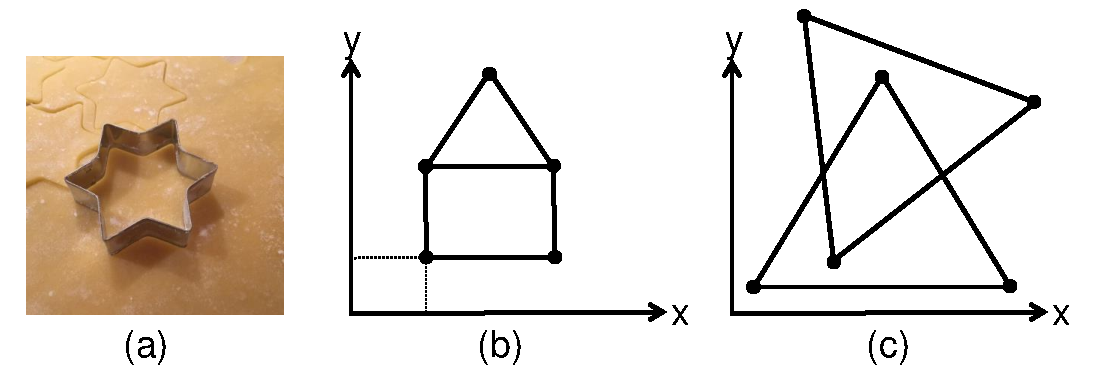
\includegraphics[width=\columnwidth]{img/CookieCAD.pdf}
\caption{Running Example CookieCAD.}%   
\label{fig:CookieCAD}

\end{figure}

%Many engineering disciplines (civil, mechanical, electrical, among others) 
%require an \emph{a priori} \emph{design}, i.e. a kind of specification, or plan, 
%of the final object, be it a bridge, a car's clutcher, or a complex electronic 
%card. From an \textsc{Mpm} viewpoint, designs play the role of \emph{models}: 
%they abstract from the real product while still possessing interesting 
%properties, making them cheaper to produce and easier to analyse. To support 
%designers, Computer-Aided Design (\textsc{Cad}) promotes the use of computers to 
%help create, modify, and analyse designs, but also optimise against known 
%constraints from a given domain. \textsc{Cad} has significantly improved many 
%engineering disciplines by improving the designs quality and increase the 
%designers' productivity, and even becoming standard development tools for 
%disciplines like electronics. \textsc{Cad} tools allow the \emph{visually} 
%design in 2D, 3D and even 4D (adding the time dimension), based on various 
%techniques such as Finite Element Methods, thus manipulating complex 
%Differential Equations. 

%For the purpose of this introductory work, we propose the Poor-Man \textsc{Cad} 
%(abbreviated as \textsc{PCad}), a (toy) (multi-)formalism that allows designing 
%2D geometric lines (noted $L$) representing arbitrary shapes, based on the 
%definition of points (noted $P$) placed on a cartesian plan (defined by integer 
%X- and Y-coordinates). When required, lines may be colored to emphasize 
%surfaces of a shape or parts of a design. Colors (noted as $C$) are encoding as 
%RGB integer triples for simplicity. The following Definition and Example 
%provides a formal specification and a visual representation of a possible 
%design.

\andreas{Fix the mathematical description with reals in Sem Dom instead of Integers.
Also, figure out some properties illustrating properties on workflows and languages.
}

\begin{Definition}[\label{def:PCAD}\textsc{Pcad} Designs] A \textsc{PCad}
object (or design) $o\in \PCAD$ is a set of lines.
A \emph{line} $l \in L$ is defined as a set of exactly two points.
A \emph{point} $p\in P$ is a pair of reals.
\begin{olddef}
Similarly, a \emph{colored} \textsc{PCad} object $o\in \PCADC$ is a set of 
lines defined over \emph{colored} points.
A \emph{color} $c\in C$ is a triple of integers corresponding to its RGB encoding.
The function $\SMapping$ maps objects $o\in \PCAD$ and $o\in \PCADC$ to the
union of points the lines constituting the objects are made of.
For the latter these points are colored.
\end{olddef}
\begin{newdef}
The function $\SMapping$ maps objects $o\in \PCAD$ to the union of points 
the lines constituting the objects are made of.
\end{newdef}

\begin{olddef}
\begin{displaymath}
\begin{small}
\begin{array}{rcl rcl}

\PCAD &\eqdef& \wp(L)                         & \PCADC &\eqdef& \wp(CL)\\
L     &\eqdef& \{ \{p, p'\} \;|\;             & 
CL    &\eqdef& \{ (\{p, p'\}, c) \;|\;  \\  
      &      & \quad p, p' \in P, p\neq p' \} & & & p, p' \in P, c\in C\}\\
P     &\eqdef& \mathbb{N} \times \mathbb{N}   & C     &\eqdef& 
{0; \ldots; 255}^3

\end{array}
\end{small}
\end{displaymath}
\end{olddef}

\begin{newdef}
\begin{displaymath}
\begin{small}
\begin{array}{rcl}
%%
\PCAD &\eqdef& \wp(L)                                       \\%& \PCADC &\eqdef& \wp(CL)\\
L     &\eqdef& \{ \{p, p'\} \;|\; p, p' \in P, p\neq p'     \\%& CL    &\eqdef& \{ \{p, p'\} \;|\;  \\  
%      &      & \quad p, p' \in P, p\neq p' \}               \\%& & & p, p' \in CP, p\neq p'\\
P     &\eqdef& \mathbb{R} \times \mathbb{R}                 \\%& CP     &\eqdef& P \times \{0; \ldots; 255\}^3
%%
\end{array}
\end{small}
\end{displaymath}
\end{newdef}

The semantics of a \textsc{Pcad} object is captured by the function 
$\SMapping$, that maps each object to the points the lines constituting the 
objects are built upon. The semantics of a colored \textsc{Pcad} object is 
similar, except that lines defined with points of different colors are 
blackened.
%%
\begin{olddef}
\begin{displaymath}
\begin{small}
\begin{array}{rcl}
%%
\SMapping & \colon & \!\!\!
\begin{array}[t]{rcl}
         \PCAD &\to& \wp(L) \\
         o &\mapsto& \bigcup o\\
\end{array}\\\\

\SMapping & \colon & \!\!\!

\begin{array}[t]{rcl}
         \PCADC &\to& (P \nrightarrow C)\\
         o &\mapsto& \left\{ \begin{array}{rclcl}
            (p, p') &\mapsto& c & \mathrm{if} & c = c'\\
            (p, p') &\mapsto& (0,0,0) & \mathrm{if} & c \neq c'\\ 
         \end{array}\right. \\
         & \multicolumn{2}{l}{\forall (\{p, p'\}, c), (\{p, p'\}, c') \in o}\\
\end{array}

\end{array}
\end{small}
\end{displaymath}
\end{olddef}
%%
\begin{newdef}
\begin{displaymath}
\begin{small}
\begin{array}{rcl}
%%
\SMapping & \colon & \!\!\!
%%
\begin{array}[t]{rcl}
%%
\PCAD &\to& \wp(\mathbb{R}^2) \\
%%
o &\mapsto& \lbrace \lbrace u,v\rbrace \;|\; \exists u,v\in \mathbb{R}.\; 
                                             \forall x \leq u \leq x'. \\
& & v{=}m{*}u{+}\left(y{-}m{*}x\right), o{=}\lbrace \lbrace x, y \rbrace, \lbrace x', y' \rbrace \rbrace,
%%
\end{array}\\
\end{array}
\end{small}
\end{displaymath}
\noindent 
where $m = \frac{y'-y}{x'-x}$ and w.l.o.g. $x' \geq x$.

\end{newdef}

\end{Definition}

\begin{olddef}
\begin{Example}[PCAD]

   Figure \ref{fig:PCAD-Visual} presents a visual representation of a very 
simple \textsc{Pcad} object. 
\begin{figure}[t]
   \centering
%    \includegraphics[width=0.98\columnwidth]{}
   \caption{A simple PCAD Object named $\mathsf{Form}$.}%
   \label{fig:PCAD-Visual}%
\end{figure}
\end{Example}

As minimal activities on \textsc{Pcad} designs, one shall evidently 
\emph{create} designs, \emph{check} for ensuring they represent valid, viable 
physical objects, and ultimately \emph{manufacture} the physical objects from 
the designs.
\end{olddef}

\begin{newdef}
As minimal activities on \textsc{Pcad} designs, one shall evidently 
\emph{create} designs, \emph{check} for ensuring they represent valid, viable 
cookie stencils, and ultimately \emph{manufacture} the stencils from 
the designs.
\end{newdef}


% \subsection{Finite-State Automata}
% \label{sec:Examples-FSM}
% 
% Finite State Automata (\textsc{Fsa}), as originally defined by Moore 
% \cite{J:Moore:1956}, link states with transitions that carry a label. 
% \textsc{Fsa} describe discrete state-based computations. Many variations of 
% \textsc{Fsa} exist together with various semantics, among which the 
% ``word-accepting'' semantics is one of the most used \cite{}. 
% 
% The \UML State Machines \cite{TR:UML-2.5:2015} is the language used by many 
% tools for expressing, among other possibilities, the behaviour of a \UML 
% object. Beyond state-based computations, \UML State Machines add several new 
% concepts like hierarchical and orthogonal states, history, and the possibility 
% to interact with the environment through outputs.
% 
% \subsection{Java}
% \label{sec:Examples-Java}
% 
% Java \cite{B:Java:2019} is a modern object-oriented programming language that 
% has become widely used for a large variety of applications. 
% 
% Wegner criteria for OO \cite{Wegner:1987}
% 
% \subsection{The \textsc{Md}$\star$ Jungle of Acronyms}
% \label{sec:Examples-MD}
% 
% \cite{B:Brambilla-Cabot-Wimmer:2012}


\begin{table}[t]
   \begin{center}
      \begin{tabular}[t]{c l}
         \hline
         \multicolumn{2}{l}{$\iota_1$: State Automata ($\mathsf{SA}$)}\\
         \hline
         SA1 & Contains the concepts of State and Transition\\
         SA2 & Possess a Transition enabler\\
         SA3 & Changes state when a transition is enabled\\
         \hline\hline
         \multicolumn{2}{l}{$\iota_2$: Object Orientation ($\mathsf{OO}$)}\\
         \hline
         OO1 & Possess the concepts of Object and Class\\
         OO2 & Objects possess a state and a set of capabilities / operations \\
         OO3 & Possess an inheritance mechanism\\
         OO4 & Inheritance allows to reuse operations\\
         \hline\hline
         \multicolumn{2}{l}{$\iota_3$: Computer-Aided Design ($\mathsf{CAD}$)}\\
         \hline
         CAD1 & Comprises concepts of (2D/3D) points and shapes\\
         CAD2 & Objects yield a position and a color\\
         CAD3 & Supports transformation into physical (2D/3D) printed objects\\
         \hline
      \end{tabular}
   \end{center}
   \label{tab:Properties}
   \caption{Properties of three paradigms: State Automata ($\mathsf{SA} 
\cite{J:Moore:1956}$); Object Orientation ($\mathsf{OO} \cite{Wegner:1987}$) 
and Computer-Aided Design ($\mathsf{CAD} \cite{}$)}
\end{table}
